% radarnet_hw_overview.tex — Fig. 2: top-level datapath of the RadarNet-1D accelerator (rn_top)
% Build: pdflatex radarnet_hw_overview.tex  →  radarnet_hw_overview.pdf
\documentclass[border=3pt]{standalone}
\usepackage{tikz}
\usetikzlibrary{positioning,arrows.meta,calc}
\begin{document}
\sffamily\footnotesize
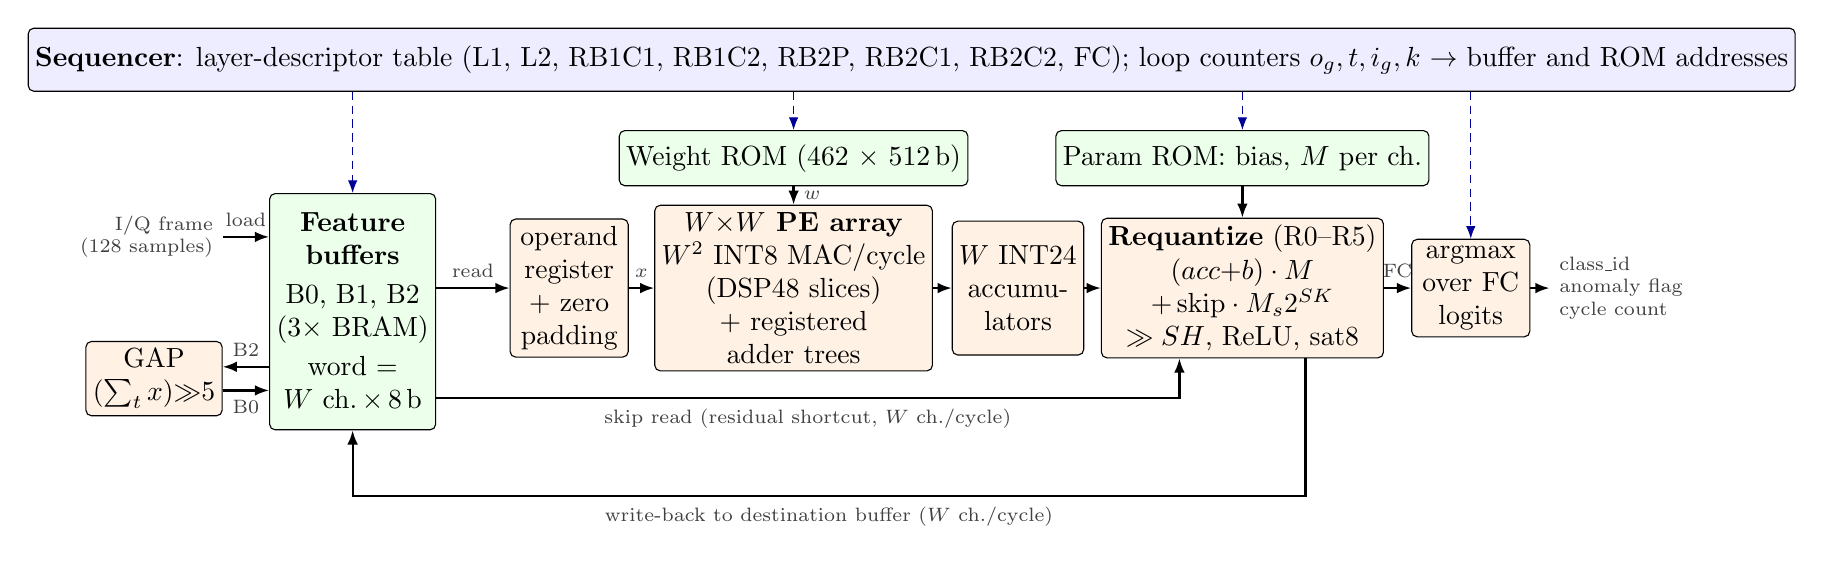
\begin{tikzpicture}[
  blk/.style={draw, rounded corners=2pt, align=center, inner sep=2.5pt, fill=white},
  mem/.style={blk, fill=green!8},
  dp/.style={blk, fill=orange!10, minimum height=17mm},
  ctl/.style={blk, fill=blue!7},
  one/.style={-{Latex[length=1.8mm]}, thick},
  ctrl/.style={-{Latex[length=1.6mm]}, densely dashed, blue!60!black},
  lbl/.style={font=\scriptsize, text=black!75}]

% ---------------- main row (y = 0.3) ----------------
\node[mem, minimum width=19mm, minimum height=30mm] (buf) at (0,0)
  {\textbf{Feature}\\ \textbf{buffers}\\[2pt] B0, B1, B2\\ (3$\times$ BRAM)\\[2pt] word $=$\\ $W$ ch.\,$\times$\,8\,b};
\node[dp, minimum width=15mm] (opr) at (2.75,0.3) {operand\\ register\\ + zero\\ padding};
\node[dp, minimum width=25mm] (pe)  at (5.6,0.3)  {\textbf{$W{\times}W$ PE array}\\ $W^2$ INT8 MAC/cycle\\ (DSP48 slices)\\ + registered\\ adder trees};
\node[dp, minimum width=15mm] (acc) at (8.45,0.3) {$W$ INT24\\ accumu-\\ lators};
\node[dp, minimum width=27mm] (rq)  at (11.3,0.3) {\textbf{Requantize} (R0--R5)\\ $(acc{+}b)\cdot M$\\ $+\,\mathrm{skip}\cdot M_s 2^{SK}$\\ $\gg SH$, ReLU, sat8};
\node[dp, minimum width=15mm, minimum height=12mm] (am) at (14.2,0.3) {argmax\\ over FC\\ logits};

\draw[one] (buf.east |- opr.west) -- node[lbl, above] {read} (opr.west);
\draw[one] (opr) -- node[lbl, above] {$x$} (pe);
\draw[one] (pe) -- (acc);
\draw[one] (acc) -- (rq);
\draw[one] (rq) -- node[lbl, above] {FC} (am);
\node[lbl, align=left, anchor=west] (out) at (15.2,0.3) {class\_id\\ anomaly flag\\ cycle count};
\draw[one] (am) -- (out);

% ---------------- ROMs ----------------
\node[mem, minimum width=25mm, minimum height=7mm] (wrom) at (5.6,1.95)  {Weight ROM (462 $\times$ 512\,b)};
\node[mem, minimum width=27mm, minimum height=7mm] (prom) at (11.3,1.95) {Param ROM: bias, $M$ per ch.};
\draw[one] (wrom) -- node[lbl, right] {$w$} (pe);
\draw[one] (prom) -- (rq);

% ---------------- sequencer ----------------
\node[ctl, minimum width=150mm, minimum height=8mm] (seq) at (7.1,3.2)
  {\textbf{Sequencer}: layer-descriptor table (L1, L2, RB1C1, RB1C2, RB2P, RB2C1, RB2C2, FC); loop counters
   $o_g, t, i_g, k$ $\rightarrow$ buffer and ROM addresses};
\foreach \n in {buf,wrom,prom,am} \draw[ctrl] (seq.south -| \n.north) -- (\n.north);

% ---------------- residual skip and write-back lanes ----------------
\coordinate (sk0) at ($(buf.east)+(0,-1.1)$);
\coordinate (sk2) at ($(rq.south)+(-0.8,0)$);
\draw[one] (sk0) -- node[lbl, below] {skip read (residual shortcut, $W$ ch./cycle)} (sk0 -| sk2) -- (sk2);
\draw[one] ([xshift=8mm]rq.south) -- ++(0,-1.75) -| node[lbl, below, pos=0.25] {write-back to destination buffer ($W$ ch./cycle)} (buf.south);

% ---------------- input and GAP ----------------
\node[lbl, align=right, anchor=east] (in) at (-1.65,0.95) {I/Q frame\\ (128 samples)};
\draw[one] (in.east) -- node[lbl, above] {load} (in.east -| buf.west);
\node[dp, minimum width=14mm, minimum height=9mm, anchor=east] (gap) at (-1.65,-0.85) {GAP\\ $(\sum_t x){\gg}5$};
\draw[one] ([yshift=1.5mm]buf.west |- gap.east) -- node[lbl, above] {B2} ([yshift=1.5mm]gap.east);
\draw[one] ([yshift=-1.5mm]gap.east) -- node[lbl, below] {B0} ([yshift=-1.5mm]buf.west |- gap.east);
\end{tikzpicture}
\end{document}
